% ==================================================================
% 4.5 Val bay that   (file: sections/12_exp_flight.tex)
% ==================================================================
\subsection{Validation on Real Flight Footage}
\label{sec:flight}

Everything above rests on a simulated corruption. This section does not: we annotated
$92$ frames from an autonomous following run at roughly $6$\,m and evaluated six models
on them under the same protocol. The blur here was produced by the aircraft, not by us.

\begin{table}[t]
\centering
\caption{Real flight footage, $92$ annotated frames at $\approx6$\,m, same evaluation
code as the other tables. Within each group the three models are architecturally
identical and differ only in the treatment, so the two effects (training domain across
groups, treatment within) are independent. Paired $95\%$ confidence intervals over
frames are reported in the text.}
\label{tab:flight}
\setlength{\tabcolsep}{5pt}
\begin{tabular}{llcccc}
\toprule
Training data & Treatment & AP$_{50}$ & AP$_{50:95}$ & AP$_{75}$ & AR$_{100}$ \\
\midrule
VisDrone + COCO person & none            & 0.7613 & 0.3369 & 0.1448 & 0.5076 \\
VisDrone + COCO person & vibration-aware & 0.7747 & 0.3792 & 0.2583 & \best{0.5315} \\
VisDrone + COCO person & consistency     & \best{0.8798} & \best{0.3885} & \best{0.2620} & 0.5087 \\
\midrule
VisDrone only          & none            & 0.1435 & 0.0547 & 0.0166 & 0.4315 \\
VisDrone only          & vibration-aware & 0.0579 & 0.0207 & 0.0076 & 0.4076 \\
VisDrone only          & consistency     & 0.0909 & 0.0283 & 0.0093 & 0.3772 \\
\bottomrule
\end{tabular}
\end{table}

% ---------------------------------------------------------------------
% Hinh dinh tinh (fig4_qualitative): TAM BO RA de vua 12 trang.
% Bang~\ref{tab:flight} da mang du bang chung dinh luong; hinh nay chi minh hoa.
% Muon dua lai: bo comment khoi duoi + doi lai caption Fig.~\ref{fig:qual}
% trong doan mo dau muc nay.
% \begin{figure}[t]
% \centering
% 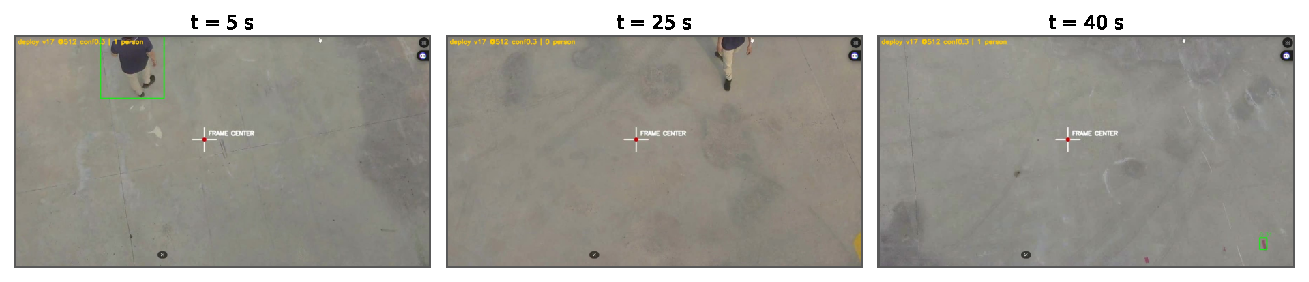
\includegraphics[width=0.82\textwidth]{figures/fig4_qualitative.pdf}
% \caption{Detections during an autonomous following run at roughly $6$\,m. Note the
% scale of the subject relative to the frame: this is the regime the VisDrone-only
% model was never supervised on, and where its localisation collapses while its
% recall holds up (Table~\ref{tab:flight}).}
% \label{fig:qual}
% \end{figure}
% ---------------------------------------------------------------------

\subsubsection{Both treatments transfer to real vibration.}
Among the models competent in this domain, both treatments improve on the untreated
baseline in the same way. AP$_{75}$ rises from $0.1448$ to $0.2583$ for
vibration-aware training and $0.2620$ for the consistency variant, relative gains of
$78$ and $81\%$ in strict-IoU localisation, while recall barely moves
($0.5076 \rightarrow 0.5315$ and $0.5087$). Neither is finding more people; both
place tighter boxes around the people they already find, the signature expected if
they had learned to resolve structure through blur. Because this corruption is
physical rather than synthetic, it is the strongest single piece of evidence that
the mechanism addresses the real degradation.

Because $92$ frames is a small sample, we resampled frames $1000$ times, paired
across models, and report $95\%$ intervals on the paired differences. Both
treatments beat the untreated baseline on AP$_{50:95}$ and AP$_{75}$ with intervals
excluding zero: $+0.042\,[+0.011, +0.074]$ and $+0.108\,[+0.010, +0.211]$ for
vibration-aware training, $+0.051\,[+0.012, +0.087]$ and
$+0.110\,[+0.012, +0.214]$ for the consistency variant.

The two treatments separate from each other on AP$_{50}$ alone,
$+0.106\,[+0.058, +0.161]$ in favour of the consistency variant, while their
AP$_{50:95}$ and AP$_{75}$ differences both straddle zero
($+0.009\,[-0.023, +0.044]$ and $+0.002\,[-0.074, +0.073]$). That AP$_{50}$ gap is
real within this footage and reverses the VisDrone-Shake ordering, where
vibration-aware training leads by $6.2$ points. We do not know which ordering
generalises. One subject in one scene at one altitude cannot decide it, and the
resolution is a larger flight set rather than a further argument from these
$92$ frames.

In the VisDrone-only group the ordering reverses, with AP$_{50}$ falling from $0.1435$
to $0.0909$, and we report this rather than omit it. Both of those models are failures
in this domain, having been supervised only on instances a few pixels across, so the
comparison is between two failure modes: making a representation invariant to blur
helps only where the representation is otherwise adequate. Vibration-consistency is a
robustness treatment, not a domain-adaptation method.

\subsubsection{Benchmark ranking inverts on the deployment condition.}
Adding COCO person images multiplies AP$_{50}$ on real footage by $5.3\times$
($0.1435 \rightarrow 0.7613$), while on VisDrone-val the same addition \emph{costs}
accuracy ($0.5127$ against $0.5016$). The mechanism is in the breakdown: the VisDrone-only model
keeps moderate recall ($0.4315$), so it does see the person, but localisation
collapses (AP$_{75}$ of $0.0166$) because it has never been supervised on a person
filling much of the frame. Selecting training data by benchmark performance would
have selected precisely the wrong model. For short-range following, training data
should match the deployment altitude band rather than the evaluation benchmark.

This set is one subject, one scene, one altitude and $92$ frames from a ground-station
capture, so it establishes the direction and rough magnitude of both effects but is not
a benchmark (Section~\ref{sec:limitations}).
